% !TEX encoding = UTF-8 Unicode
\documentclass[12pt]{article}
\usepackage[english,greek]{babel}
\usepackage[utf8x]{inputenc}
\usepackage{amssymb,latexsym,amsmath,ucs,amsthm,setspace,graphicx}
\usepackage{kerkis}
\usepackage{tikz}
\usepackage{algorithm2e}

\newcommand{\HRule}{\rule{\linewidth}{0.5mm}}


\begin{document}
\begin{titlepage}
\centering


\includegraphics[scale=0.3]{pyrforos.jpg}

\textsc{\LARGE Σχολή \\ Ηλεκτρολόγων Μηχανικών \\[-3pt] και \\[6pt] Μηχανικών Υπολογιστών}

\vspace{1cm}

% Title
\HRule \\[0.4cm]
{\huge \bfseries Λειτουργικά Συστήματα\\} %\\

\vspace{0.4cm}
\HRule \\[0.4cm]

\Large{2η σειρά ασκήσεων}



% Authors
\vfill
\begin{center}
\large
%Add authors one after another with the same format

Ομάδα \textlatin{oslabb12} 

Γκούμας Βασίλης ---  03113031 

Ζαρίφης Νικόλαος --- 03112178

%\vfill
\end{center}

\end{titlepage}



\section*{Άσκηση 1}

Ο πηγαίος κώδικας βρίσκεται στο αρχείο \textlatin{ask2-fork.c} και παρακάτω βλέπουμε το  \textlatin{output} της εκτέλεσης του. Όπως θα δούμε και στα θεωρητικά ερωτήματα, η παραπάνω έξοδος παράχθηκε με \textlatin{show\_pstree(getpid())}.

 Στη περίπτωση που είχαμε  \textlatin{show\_pstree(pid)} θα έιχαμε το ίδιο αποτέλεσμα στο δέντρο, χωρίς όμως την γραμμή που περιέχει τα \textlatin{sh, pstree}

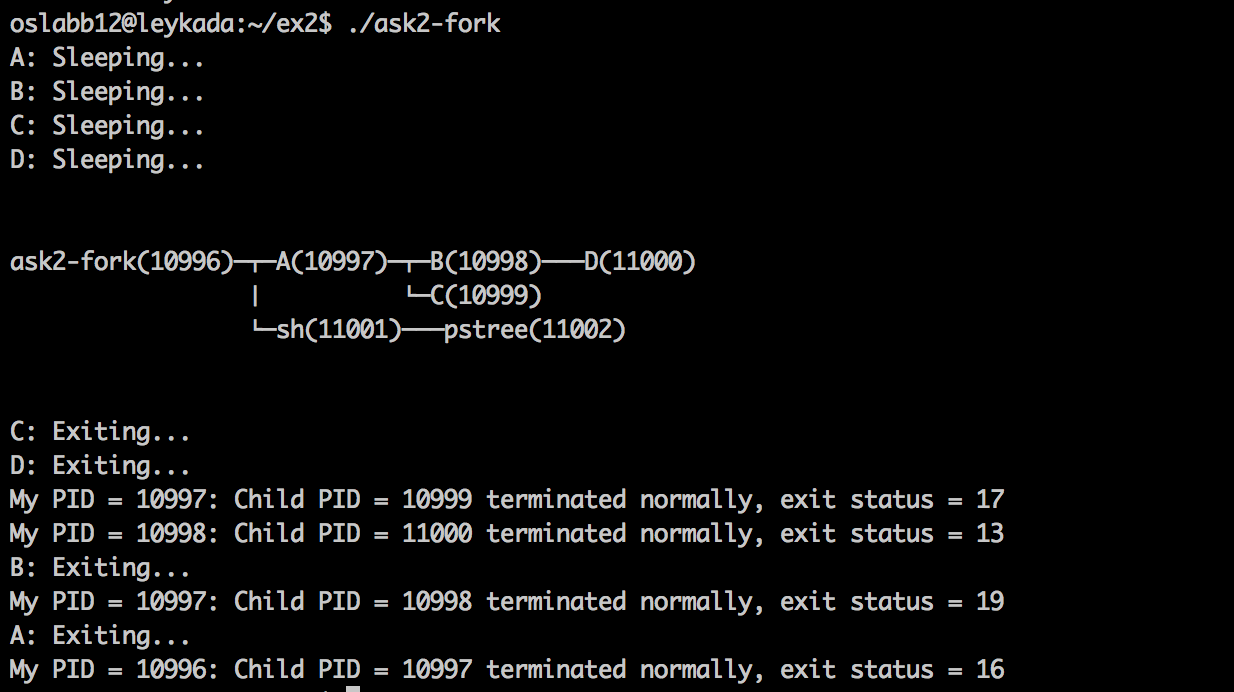
\includegraphics[scale=0.5]{ask2-fork.png}

\subsection*{1ο ερώτημα }
'Αμα τερματίσουμε πρόωρα μια διεργασία, τότε όλα τα παιδιά θα περάσουν σε μια κατάσταση που ονομάζεται \textlatin{zombie}  καθώς δεν θα υπάρχει ο γονιός για να τα κάνει \textlatin{wait}. Σε αυτή την περίπτωση , η πρακτική που ακολουθείται στα $unix$ λειτουργικά συστήματα είναι τα παιδιά \textlatin{zombies} να γίνονται παιδιά μιας διεργασίας με $pid=1$, η οποία κάνει διαρκώς \textlatin{wait}.

\subsection*{2ο ερώτημα}

Γράφοντας \textlatin{show\_ps\_tree(getpid())} αντί για \textlatin{show\_ps\_tree(pid)}, θα εμφανιστεί το δέντρο συμπεριλαμβάνοντας την διεργασία του προγράμματός μας (\textlatin{ask2-fork} ), η οποία κάνει \textlatin{fork} μια διεργασία \textlatin{shell} η οποία με τη σειρά της καλεί την \textlatin{pstree} που εκτυπώνει το ζητούμενο δέντρο.


\subsection*{3ο ερώτημα}

Αν ο διαχειριστής δεν έχει θέσει όριο στον αριθμό διεργασιών που μπορεί να δημιουργήσει ένας χρήστης τότε είναι πιθανό λόγω κακής/κακόβουλης χρήσης να εξαντληθούν οι πόροι του μηχανήματος, καθιστώντας το αχρησιμοποιήτο απο τους υπόλοιπους χρήστες. Χαρακτηριστικό παράδειγμα κακόβουλης χρήσης είναι το \textlatin{forkbomb} που είναι μια συνάρτηση που συνεχώς κάνει \textlatin{fork} τον εαυτό της.


\section*{'Ασκηση 2}

Ο κώδικας της άσκησης βρίσκεται στο αρχείο \textlatin{ask2-tree.c}. Επίσης περιέχονται μερικά \textlatin{testcases} που τρέξαμε με όνομα \textlatin{*.in} και \textlatin{*.out} αντίστοιχα καθώς και το \textlatin{output} της εκτέλεσής του. 

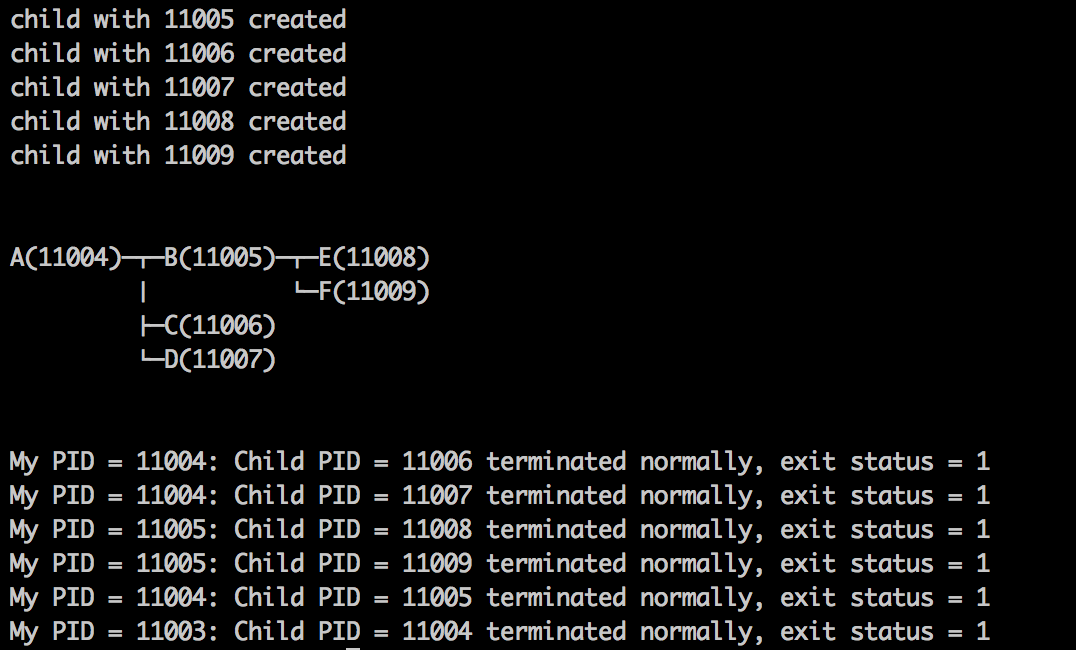
\includegraphics[scale=0.5]{ask2-tree.png}

\subsection*{Ερώτημα 1ο}

Όπως βλέπουμε τα μηνύματα έναρξης εμφανίζονται κατα βάθος \textlatin{bfs}, καθώς κάθε διεργασία δημιουργεί με ένα \textlatin{for} τα παιδιά της.Τα μηνύματα τερματισμού αντίστοιχα, δεν έχουν κάποιο μοτίβο, καθώς χωρίς επιπλέον έλεγχο η σειρά που θα εμφανιστούν εξαρτάται απο τη σειρά που θα δώσει ο \textlatin{scheduler} στις διεργασίες.



\section*{'Ασκηση 3}

Ο κώδικας της άσκησης βρίσκεται στο αρχείο \textlatin{ask2-signals.c}

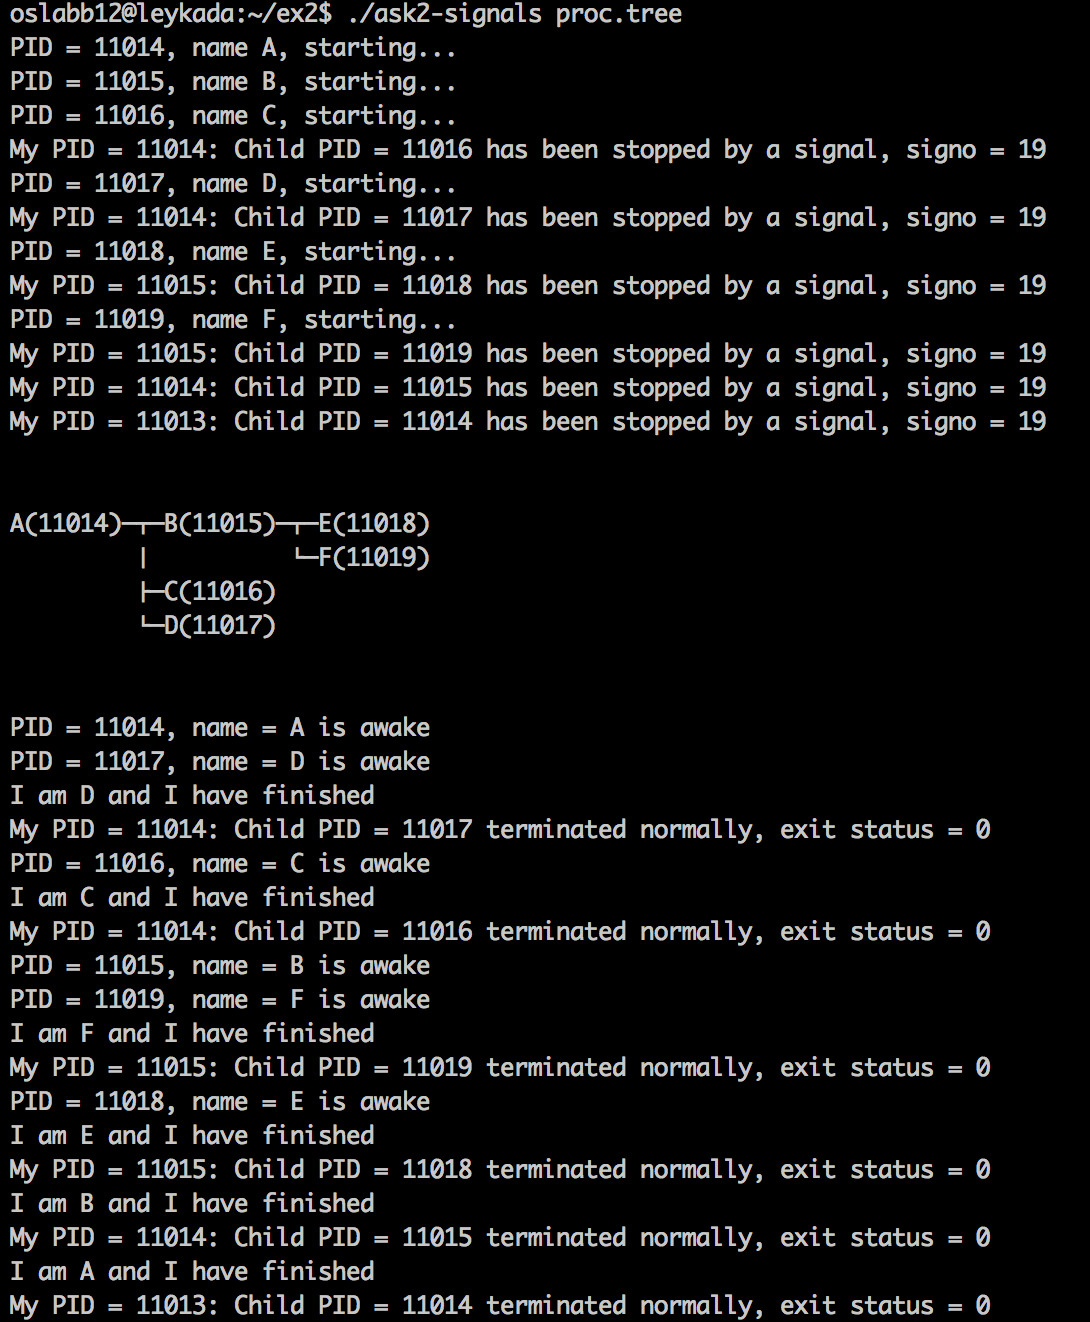
\includegraphics[scale=0.5]{ask2-signals.png}


\subsection*{1ο ερώτημα}

Στις ασκήσεις 1 και 2 που έγινε χρήση της \textlatin{sleep()}, χρειάστηκε να περιμένουμε ένα χρονικό διάστημα που εμείς 
ορίζουμε εκ των προτέρων, το οποίο υπολογίζουμε ότι θα είναι αρκετό για να δημιουργηθεί ολόκληρο το δέντρο διεργασιών,
πριν το τυπώσουμε.

Προφανώς αυτή η διαδικασία δεν είναι αρκετή για σε περίπτωση που το δέντρο διεργασιών γίνεται μεγάλο καθώς δεν κάνει \textlatin{scale}
και απαιτεί περιττή δουλειά απο τον προγραμματιστή.
και γενικά όταν θέλουμε να κάνουμε ακριβή συγχρονισμό διεργασιών.

Χρησιμοποιώντας σήματα έχουμε μεγαλύτερο έλεγχο στον συγχρονισμό καθώς ξυπνάμε και κοιμίζουμε τις διεργασίες ακριβώς τη στιγμή που τις χρειαζόμαστε, έχοντας ταυτόχρονα πετύχει ασύγχρονο τρόπο επικοινωνίας μεταξύ των δεργασιών.

\subsection*{2ο ερώτημα}

Όπως βλέπουμε και απο την υλοποίηση της, η \textlatin{wait\_for\_ready\_children()} σιγουρεύεται πως όλα τα παιδιά της εκάστοτε 
διεργασίας που την κάλεσε, έχουν γίνει \textlatin{pause} και δεν έχουν τερματίσει για κάποιον άλλο λόγο.

Αυτό το καταφέρνει εξετάζοντας τη κατάσταση τερματισμού μέσω των τιμών που επιτρέφει η \textlatin{waitpid()} και συγκεκριμένα μέσω του \textlatin{WIFSTOPPED(status)}. 

Στο πρόγραμμά μας, η \textlatin{wait\_for\_ready\_children} καλείται αναδρομικά για κάθε παιδί και στη συνέχεια κάνουν \textlatin{pause} τον εαυτό τους. Επομένως η κλήση της \textlatin{wait\_for\_ready\_children} που βρίσκεται στη \textlatin{main}, περιμένει να σχηματιστεί ολόκληρο το δέντρο πριν καλεστεί η συνάρτηση που θα το τυπώσει. 

Η χρήση της εξασφαλίζει ότι γνωρίζουμε την κατάσταση του δέντρου πριν προσπαθήσουμε να ξυπνήσουμε παιδιά τα οποία ενδεχομένως να μην έχουν γίνει ακόμα \textlatin{pause} ή να μην έχουν καν δημιουργηθεί.


\section*{'Ασκηση 4}

Ο κώδικας της άσκησης βρίσκεται στο \textlatin{ask2-pipes.c}
Παρακάτω φαίνεται το αποτέλεσμα του προγράμματός μας για το \textlatin{testcase} που μας δώθηκε.

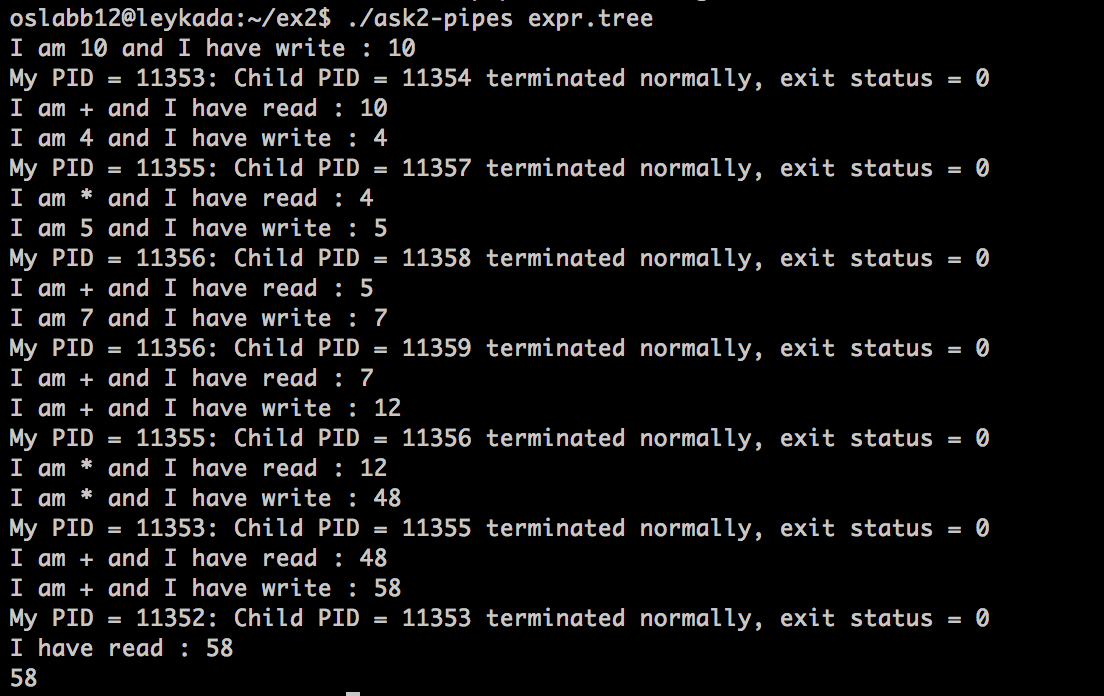
\includegraphics[scale=0.5]{ask2-pipes.png}


\subsection*{1ο ερώτημα}

Στο πρόγραμμα μας κάθε διεργασία αλληλεπιδρά με δύο σωληνώσεις, με αυτή που γράφει και με αυτή που διαβάζει. Εξαίρεση βέβαια αποτελούν οι ακραίες διεργασίες, τα φύλλα μόνο γράφουν το αποτέλεσμα τους ώστε να το μεταβιβάσουν σε μεγλύτερο επίπεδο, ενώ η ρίζα απλά διαβάζει το αποτέλεσμα απο τις γονικές της διεργασίες και το τυπώνει.

Για την επικοινωνία της γονικής διεργασίας με τα παιδιά της, χρησιμοποιήθηκε ένα \textlatin{pipe}, το οποίο μοιράζονται τα δύο παιδιά.Στη συγκεκριμένη περίπτωση το κοινό  \textlatin{pipe} για τα παιδιά είναι υλοποιήσιμο καθώς δεν χρειάζετε να ξέρουμε ποιο αποτέλεσμα προήλθε απο ποιο παιδί, καθώς η πράξη της πρόσθεσης και του πολλαπλασιασμού είναι αντιμεταθετικές.

Επομένως στη γενική περίπτωση, όπως πχ στην πράξη της αφαίρεσης, ή οποιασδήποτε λειτουργία απαιτεί να ξέρουμε απο ποιο παιδί ήρθε κάποιο αποτέλεσμα, θα αναγκαστούμε να χρησιμοποήσουμε ένα \textlatin{pipe} ανα παιδί, είτε να παρακαλοθούμε πότε τερματίζει κάθε παιδί.


\subsection*{2ο ερώτημα}

Σε ένα πολυεπεξεργαστικό σύστημα, οι διαφορετικές διεργασίες/\textlatin{thread} που δημιουργούμε για τους κόμβους, είναι δυνατόν να εκτελούνται σε διαφορετικές \textlatin{cpu}, με αποτέλεσμα να επιτυγχάνεται παραλληλοποίηση και να έχουμε \textlatin{performance boost} και αρκετά γρηγορότερο χρόνο εκτέλεσης.

Για να έχουμε όσο δυνατόν μεγαλύτερο όφελος απο την παραλληλοποίηση, θα πρέπει το πρόγραμμα μας να μπορεί να διαχωριστεί σε τμήματα με χαμηλά ή μηδαμινά \textlatin{dependencies}.

Για το παράδειγμα μας, μια περίπτωση εκφυλισμού όπου η παράλληλη εκτέλεση είναι ισοδύναμη με την σειριακή είναι όταν επιτρέπεται η χρήση παρενθέσεων. Στη συγκεκριμένη περίπτωση, μπορεί ένα απο καιρό έτοιμο αποτέλεσμα να \textlatin{stall}άρει καθώς αναμένει αποτέλεσμα απο τις \textlatin{nested} παρενθέσεις. Το δέντρο της διεργασίας στην παραπάνω περίπτωση θα ήταν εντελώς \textlatin{imbalanced} προς τα δεξιά ή αριστερά. Αντίθετα, όσο πιο κοντά είμαστε σε πλήρες δέντρο, τόσο μειώνονται τα \textlatin{dependencies} και έχουμε μεγαλύτερο όφελος απο την παραλληλία.


\section*{Προαιρετικές}

\subsection*{1ο ερώτημα}

Όπως είδαμε και στο 2ο ερώτημα της 4ης άσκησης, ο χρόνος υπολογισμού μιας αριθμητικής έκφρασης εξαρτάται απο τη μορφή του δέντρου.Όσο πιο κοντά σε πλήρες είναι το δέντρο μας, τόσο μεγαλύτερο \textlatin{speedup} έχουμε απο την παραλληλοποιήση και χρόνος εκτέλεσης προσεγγίζει το \textlatin{O(logn)}, όπου \textlatin{n} το πλήθος των κόμβων του δέντρου.Αν το δέντρο εκφυλίζεται προς τα αριστερά/δεξιά τότε ο χρόνος εκτέλεσης τείνει να γίνει \textlatin{O(n)} .

 Άμα έχουμε ένα δέντρο με \textlatin{n} κόμβους, το οποίο είναι κατα προσέγγιση πλήρες, τότε το μέγιστο πλήθος ταυτόχρονων διεργασιών που θα τρέξουν είναι \textlatin{n} επομένως δεν έχει νόημα να προσθέσουμε περισσότερους επεξεργαστές. Επομένως χρησιμοποιώντας \textlatin{n} επεξεργαστές μπορούμε να πετύχουμε ιδανικό \textlatin{speedup} χωρίς να μένει ανεξυπηρέτητος κάποιος κόμβος.Περισσότεροι επεξεργαστές δεν θα αξιοποιηθούν και επομένως αποτελούν σπατάλη πόρων.Λιγότεροι ίσως βρεθούν σε κατάσταση που είναι όλοι απασχολημένοι και κάποια διεργασία περιμένει να τρέξει.
 

 
 \subsection*{2o ερώτημα}
 
 Το πλεονέκτημα της υβριδικής υλοποίησης είναι ότι δε δεσμεύει επεξεργαστές που υπάρχει περίπτωση να βρίσκονται σε κατάσταση αναμονής, αν υπάρχουν μεγάλα \textlatin{dependencies}.
 
 Αυξάνοντας το μ έχουμε βελτίωση απόδοσης, με την προυπόθεση ότι στο νέο βάθος το δέντρο μας συνεχίζει να είναι κατα προσέγγιση πλήρες.
 
 Με μικρότερο μ απο την άλλη πλευρά είναι πιθανό να έχουμε μειωμένο χρόνο εκτέλεσης καθώς δεν αξιοποιούμε την παραλληλία της έκφρασης.
 
 Το βάθος ενός πλήρους δυαδικού δέντρου με \textlatin{n} κόμβους είναι \textlatin{log(n)}. Επομένως μέχρι αυτό το επίπεδο περιμένουμε να έχουμε ένα σχετικά μη εκφυλλισμένο δέντρο. Σε μεγαλύτερο βάθος περιμένουμε να έχουμε αυξημένο \textlatin{nesting} και επομένως δεν υπάρχει όφελος στην παραλληλία.


\end{document}

